\chapter{Розв'язання задачі ітеративним алгоритмом найближчих точок}

У третьому розділі наведено розв'язання поставленої задачі за допомогою
ітеративного алгоритму найближчих точок.
Досліджено збіжність алгоритму.
Перевірено однозначність оцінок, які дає алгоритм, та знайдено їх розподіл.
Представлено практичні результати застосування ітеративного алгоритму найближчих
точок із зазначенням вхідних даних.

\section{Ітеративний алгоритм найближчих точок}

Ітеративний алгоритм найближчих точок (Iterative Closest Points, ICP) \cite{icp}
складається з двох кроків, що чергуються.
Ініціюється алгоритм одиничною матрицею повороту $R = I$
та нульовим вектором зсуву $ \boldsymbol{b} = \boldsymbol{0}$.
Перший крок полягає в пошуку такої розмітки $k \, : \, S \to T$, щоб
\begin{equation}\label{eq:labeling}
 \sum \limits_{\boldsymbol{s} \in S}
  \left \Vert R \cdot \boldsymbol{s} + \boldsymbol{b} - \boldsymbol{k_s} \right \Vert^2 \to
  \min \limits_{k},
\end{equation}
де $R$ і $ \boldsymbol{b}$ фіксовані,
$k$~---~сюр'єктивне відображення із $S$ в $T$.
На наступному кроці виконується пошук повороту $R$ та зсуву $ \boldsymbol{b}$
за поточною розміткою $k$
\begin{equation}\label{eq:second:iteration}
 \sum \limits_{\boldsymbol{s} \in S}
  \left \Vert R \cdot \boldsymbol{s} + \boldsymbol{b} - \boldsymbol{k_s} \right \Vert^2
 \to \min \limits_{R, \boldsymbol{b}}.
\end{equation}
При цьому матриця $R \in SO \left( 3 \right) $,
тобто ортогональна матриця розмірності $3 \times 3$ з визначником $+1$.

\subsection{Пошук розмітки}

Розв'язання оптимізаційної задачі \eqref{eq:labeling}
зводиться до пошуку такого набору
$ \left\{ \boldsymbol{k_s} \; \middle| \; \boldsymbol{s} \in S \right\} $, щоб
\begin{equation*}
  \sum \limits_{\boldsymbol{s} \in S}
    \left \Vert R \boldsymbol{s} + \boldsymbol{b} - \boldsymbol{k_s} \right \Vert^2 \to
  \min \limits_{\boldsymbol{k_s}}.
\end{equation*}
Запишемо суму явно (нехай множина $S$ має $n$ точок)
\begin{equation*}
  \left \Vert R \cdot \boldsymbol{s_1} + \boldsymbol{b} - \boldsymbol{k_{s_1}} \right \Vert^2 +
  \dotsc +
  \left \Vert
    R \cdot \boldsymbol{s}_n + \boldsymbol{b} - \boldsymbol{k_{s_n}}
  \right \Vert^2 \to
  \min \limits_{\boldsymbol{k_{s_1}}, \boldsymbol{k_{s_2}}, \dotsc, \boldsymbol{k_{s_n}} \in T}.
\end{equation*}
Параметри, що входять у кожний доданок, різні,
тож мінімізація всієї суми еквівалентна мінімізації кожного доданку окремо
\begin{align*}
  \left\{ \begin{array}{ccc}
    \left \Vert R \cdot \boldsymbol{s_1} + \boldsymbol{b} - \boldsymbol{k}_{s_1} \right \Vert^2
    \to \min \limits_{\boldsymbol{k_{s_1}} \in T}, \\
    \left \Vert R \cdot \boldsymbol{s_2} + \boldsymbol{b} - \boldsymbol{k}_{s_2} \right \Vert^2 \to
    \min \limits_{\boldsymbol{k_{s_2}} \in T}, \\
    \vdots \\
    \left \Vert
      R \cdot \boldsymbol{s_n} + \boldsymbol{b} - \boldsymbol{k}_{s_n}
    \right \Vert^2 \to
    \min \limits_{\boldsymbol{k_{s_n}} \in T}.
  \end{array} \right.
\end{align*}
Таким чином, для кожної точки $ \boldsymbol{s} \in S$ знаходимо точку
$ \boldsymbol{t}^* \in T$ таку,
щоб відстані між парами $R \cdot \boldsymbol{s} + \boldsymbol{b}$ та $ \boldsymbol{t}^*$ для всіх
$ \boldsymbol{s} \in S$ були найменшими
\begin{equation*}
  \left \Vert R \cdot \boldsymbol{s} + \boldsymbol{b} - \boldsymbol{t}^* \right \Vert^2 =
  \min \limits_{\boldsymbol{t} \in T}
    \left \Vert R \boldsymbol{s} + \boldsymbol{b} - \boldsymbol{t} \right \Vert^2.
\end{equation*}
Якщо для якоїсь точки $\boldsymbol{s}$ знайдено декілька таких точок $\boldsymbol{t}^*$,
то вибираємо будь-яку.

\subsection{Пошук перетворення за допомогою сингулярного розкладу}

Обчислимо зсув $ \boldsymbol{b}$.
Нехай $R$~---~відома.
Мінімізуємо
\begin{equation*}
  E \left( \boldsymbol{b} \right) =
  \sum \limits_{\boldsymbol{s} \in S}
    \left \Vert R \cdot \boldsymbol{s} + \boldsymbol{b} - \boldsymbol{k_s} \right \Vert^2.
\end{equation*}
Можемо знайти оптимальний зсув,
взявши градієнт від $E$ по $ \boldsymbol{b}$ та прирівнявши його до нуля
\begin{equation}\label{eq:derivative}
  0 =
  \nabla E \left( \boldsymbol{b} \right) =
  \sum \limits_{\boldsymbol{s} \in S}
    2 \left( R \cdot \boldsymbol{s} + \boldsymbol{b} - \boldsymbol{k_s} \right) =
  2 \boldsymbol{b} \cdot \left| S \right| +
  2 R \sum \limits_{\boldsymbol{s} \in S} \boldsymbol{s} -
  2 \sum \limits_{\boldsymbol{s} \in S} \boldsymbol{k_s}.
\end{equation}
Позначимо
\begin{equation*}
  \overline{\boldsymbol{s}} =
  \frac{ \sum \limits_{\boldsymbol{s} \in S} \boldsymbol{s}}{ \left| S \right| }, \,
  \overline{\boldsymbol{k}}_{\boldsymbol{s}} =
  \frac{ \sum \limits_{\boldsymbol{s} \in S} \boldsymbol{k_s}}{ \left| S \right| }.
\end{equation*}
Перепишемо рівняння \eqref{eq:derivative} в термінах введених позначень
\begin{equation}\label{eq:translation}
  \boldsymbol{b} =
  \overline{\boldsymbol{k}}_{\boldsymbol{s}} - R \cdot \overline{\boldsymbol{s}}.
\end{equation}
Знайшли оптимальний вектор $ \boldsymbol{b}$,
який однозначно обчислюється за матрицею повороту $R$.
Підставимо його у вираз \eqref{eq:second:iteration}
\begin{equation*}
  \begin{gathered}
    \sum \limits_{\boldsymbol{s} \in S}
      \left \Vert R \cdot \boldsymbol{s} + \boldsymbol{b} - \boldsymbol{k_s} \right \Vert^2 =
    \sum \limits_{\boldsymbol{s} \in S}
      \left \Vert
        R \cdot \boldsymbol{s} + \left(
          \overline{\boldsymbol{k}}_{\boldsymbol{s}} - R \cdot \overline{\boldsymbol{s}}
        \right) - \boldsymbol{k_s}
      \right \Vert^2 = \\
    = \sum \limits_{\boldsymbol{s} \in S}
      \left \Vert
        R \cdot \left( \boldsymbol{s} - \overline{\boldsymbol{s}} \right) -
        \left( \boldsymbol{k_s} - \overline{\boldsymbol{k}}_{\boldsymbol{s}} \right)
      \right \Vert^2.
  \end{gathered}
\end{equation*}
Таким чином, в задачі мінімізації позбулися невідомого вектора $\boldsymbol{b}$,
тому залишилось знайти лише матрицю $R$.
Нехай $\tilde{\boldsymbol{s}} = \boldsymbol{s} - \overline{\boldsymbol{s}}, \,
  \tilde{\boldsymbol{k_s}} = \boldsymbol{k_s} - \overline{\boldsymbol{k}}_{\boldsymbol{s}}$,
тоді
\begin{equation}\label{eq:R}
  R =
  \arg \min \limits_{R \in SO \left( 3 \right) }
    \sum \limits_{\boldsymbol{s} \in S}
      \left \Vert R \cdot \tilde{\boldsymbol{s}} - \tilde{\boldsymbol{k_s}} \right \Vert^2.
\end{equation}
Спростимо вираз, який мінімізується в \eqref{eq:R},
використавши ортогональність матриці $R$: $R^T = R^{-1}$
\begin{equation*}
  \begin{gathered}
    \left \Vert R \cdot \tilde{\boldsymbol{s}} - \tilde{\boldsymbol{k_s}} \right \Vert^2 =
    \left( R \cdot \tilde{\boldsymbol{s}} - \tilde{\boldsymbol{k_s}} \right)^T \cdot
    \left( R \cdot \tilde{\boldsymbol{s}} - \tilde{\boldsymbol{k_s}} \right) = \\
    = \left( \tilde{\boldsymbol{s}}^T \cdot R^T - \tilde{\boldsymbol{k_s}}^T \right) \cdot
    \left( R \cdot \tilde{\boldsymbol{s}} - \tilde{\boldsymbol{k_s}} \right) = \\
    = \tilde{\boldsymbol{s}}^T \cdot R^T \cdot R \cdot \tilde{\boldsymbol{s}} -
    \tilde{\boldsymbol{k_s}} \cdot \tilde{\boldsymbol{s}}^T \cdot R \cdot \tilde{\boldsymbol{s}} -
    \tilde{\boldsymbol{s}}^T \cdot R^T \cdot
    \tilde{\boldsymbol{k_s}} + \tilde{\boldsymbol{k_s}}^T \cdot \tilde{\boldsymbol{k_s}} = \\
    = \tilde{\boldsymbol{s}}^T \cdot \tilde{\boldsymbol{s}} -
    \tilde{\boldsymbol{k_s}}^T \cdot R \cdot \tilde{\boldsymbol{s}} -
    \tilde{\boldsymbol{s}}^T \cdot R^T \cdot \tilde{\boldsymbol{k_s}} +
    \tilde{\boldsymbol{k_s}}^T \cdot \tilde{\boldsymbol{k_s}}.
  \end{gathered}
\end{equation*}

Помітимо,
що $ \tilde{\boldsymbol{s}}^T \cdot R^T \cdot \tilde{\boldsymbol{k_s}} $~---~це скаляр:
$ \tilde{\boldsymbol{s}}^T$ має розмірність $1 \times 3, \, R^T$ має розмірність
$3 \times 3$, а $ \tilde{\boldsymbol{k_s}}$ має розмірність $3 \times 1$.
Для будь-якого скаляру $a = a^T$, тому
\begin{equation*}
  \tilde{\boldsymbol{s}}^T \cdot R^T \cdot \tilde{\boldsymbol{k_s}} =
  \left( \tilde{\boldsymbol{s}}^T \cdot R^T \cdot \tilde{\boldsymbol{k_s}} \right)^T =
  \tilde{\boldsymbol{k_s}}^T \cdot R \cdot \tilde{\boldsymbol{s}}.
\end{equation*}
Маємо
\begin{equation*}
  \left \Vert R \cdot \tilde{\boldsymbol{s}} - \tilde{\boldsymbol{k_s}} \right \Vert^2 =
  \tilde{\boldsymbol{s}}^T \cdot \tilde{\boldsymbol{s}} -
  2 \tilde{\boldsymbol{k_s}}^T \cdot R \cdot \tilde{\boldsymbol{s}} +
  \tilde{\boldsymbol{k_s}}^T \cdot \tilde{\boldsymbol{k_s}}.
\end{equation*}
Підставимо отриманий вираз у \eqref{eq:R},
відкинувши суми $ \tilde{\boldsymbol{s}}^T \cdot \tilde{\boldsymbol{s}}$ та
$ \tilde{\boldsymbol{k_s}}^T \cdot \tilde{\boldsymbol{k_s}}$ по всім $\boldsymbol{s} \in S$,
бо ці вирази не залежать від $R$ та не впливають на мінімізацію
\begin{equation*}
  \begin{gathered}
    R =
    \arg \min \limits_{R \in SO \left( 3 \right) }
      \sum \limits_{\boldsymbol{s} \in S}
        \left(
          \tilde{\boldsymbol{s}}^T \cdot \tilde{s} -
          2 \tilde{\boldsymbol{k_s}}^T \cdot R \cdot \tilde{\boldsymbol{s}} +
          \tilde{k}_s^T \cdot \tilde{\boldsymbol{k_s}}
        \right) = \\
    = \arg \min \limits_{R \in SO \left( 3 \right) }
      \left(
        \sum \limits_{\boldsymbol{s} \in S} \tilde{s}^T \cdot \tilde{\boldsymbol{s}} -
        2 \sum \limits_{\boldsymbol{s} \in S}
          \tilde{\boldsymbol{k_s}}^T \cdot R \cdot \tilde{\boldsymbol{s}} +
        \sum \limits_{\boldsymbol{s} \in S} \tilde{\boldsymbol{k_s}} \cdot \tilde{\boldsymbol{k_s}}
      \right) = \\
    = \arg \min \limits_{R \in SO \left( 3 \right) } \left(
      -2 \sum \limits_{\boldsymbol{s} \in S} \tilde{\boldsymbol{k_s}}^T \cdot R \cdot
      \tilde{\boldsymbol{s}}
    \right).
  \end{gathered}
\end{equation*}
Те саме справедливо для константи, на яку множиться сума.
Також слід зазначити,
що максимізація виразу еквівалентна його мінімізації зі знаком <<мінус>>
\begin{equation*}
   R =
   \arg \max \limits_{R \in SO \left( 3 \right) }
    \sum \limits_{\boldsymbol{s} \in S}
      \tilde{\boldsymbol{k_s}}^T \cdot R \cdot \tilde{\boldsymbol{s}}.
\end{equation*}
Помітимо, що
\begin{equation*}
  \sum \limits_{\boldsymbol{s} \in S}
    \tilde{\boldsymbol{k_s}}^T \cdot R \cdot \tilde{\boldsymbol{s}} =
  tr \left( \tilde{K}^T \cdot R \cdot \tilde{S} \right),
\end{equation*}
де $ \tilde{K}$ і $ \tilde{S}$~---~це матриці розмірності $3 \times n$
зі стовпцями $ \tilde{\boldsymbol{s}}$ та $ \tilde{\boldsymbol{k_s}}$ відповідно
\begin{equation*}
  \begin{gathered}
    \tilde{K}^T \cdot R \cdot \tilde{S} =
    \begin{bmatrix}
      \tilde{\boldsymbol{k_{s_1}}}^T \\
      \tilde{\boldsymbol{k_{s_2}}}^T \\
      \vdots \\
      \tilde{\boldsymbol{k_{s_n}}}^T
    \end{bmatrix} \cdot R \cdot
    \begin{bmatrix}
      \tilde{\boldsymbol{s_1}} & \tilde{\boldsymbol{s_2}} & \dotsc & \tilde{\boldsymbol{s_n}}
    \end{bmatrix}.
  \end{gathered}
\end{equation*}
Слід квадратної матриці дорівнює сумі її діагональних елементів.
Шукаємо таку матрицю $R$, яка буде максимізувати вираз
$tr \left( \tilde{K}^T \cdot R \cdot \tilde{S} \right) $.
Слід матриці має властивість \cite{trace:fukugana}
\begin{equation}\label{eq:trace}
  tr \left( A \cdot B \right) =
  tr \left( B \cdot A \right)
\end{equation}
для будь-яких матриць $A$ та $B$ сумісних розмірностей.

Доведемо цю властивість.
Нехай матриця $A$ має розмірність $n \times m$, а матриця $B$~---~$m \times n$.
Тоді матриця $C = A \cdot B$~---~матриця розмірності $n \times n$,
що складається з елементів
\begin{equation*}
  c_{ij} =
  \sum \limits_{r = 1}^m a_{ir} \cdot b_{rj}.
\end{equation*}
Аналогічно,
матриця $D = B \cdot A$ має розмірність $m \times m$ і складається з елементів
\begin{equation*}
  d_{ij} =
  \sum \limits_{r = 1}^n b_{ir} \cdot a_{rj}.
\end{equation*}
Діагональні елементи матриць $C$ та $D$ мають вигляд
\begin{equation*}
  \begin{cases}
    c_{ii} = \sum \limits_{r = 1}^m a_{ir} \cdot b_{ri}, \\
    d_{ii} = \sum \limits_{r = 1}^n b_{ir} \cdot a_{ri}.
  \end{cases}
\end{equation*}
Запишемо слід для добутків
\begin{equation*}
  \begin{gathered}
    tr \left( A \cdot B \right) = tr \left( C \right) = \sum \limits_{i = 1}^n c_{ii} =
    \sum \limits_{i = 1}^n \sum \limits_{r = 1}^m a_{ir} \cdot b_{ri}, \\
    tr \left( B \cdot A \right) = tr \left( D \right) = \sum \limits_{i = 1}^m d_{ii} =
    \sum \limits_{i = 1}^m \sum \limits_{r = 1}^n b_{ir} \cdot a_{ri}.
  \end{gathered}
\end{equation*}
Дві отримані суми однакові.
Це означає, що $tr \left( A \cdot B \right) = tr \left( B \cdot A \right) $.

Таким чином,
\begin{equation*}
  tr \left( \tilde{K}^T \cdot R \cdot \tilde{S} \right) =
  tr \left( \tilde{K}^T \cdot \left[ R \cdot \tilde{S} \right] \right) =
  tr \left( R \cdot \tilde{S} \cdot \tilde{K}^T \right).
\end{equation*}
Позначимо
\begin{equation*}
  \begin{gathered}
    X =
    \tilde{S} \cdot \tilde{K}^T =
    \sum \limits_{i = 1}^n \tilde{\boldsymbol{s_i}} \cdot \tilde{\boldsymbol{k_{s_i}}}^T =
    \sum \limits_{i = 1}^n
      \tilde{\boldsymbol{s_i}} \cdot \left( \boldsymbol{k_{s_i}} - \overline{\boldsymbol{k}}_{\boldsymbol{s}} \right)^T = \\
    = \begin{bmatrix}
      \sum \limits_{i = 1}^n \tilde{\boldsymbol{s_i}}_x \cdot \tilde{\boldsymbol{k_{s_i}}}_x^T & \sum \limits_{i = 1}^n \tilde{\boldsymbol{s_i}}_x \cdot \tilde{\boldsymbol{k_{s_i}}}_y^T & \sum \limits_{i = 1}^n \tilde{\boldsymbol{s_i}}_x \cdot \tilde{\boldsymbol{k_{s_i}}}_z^T \\
      \sum \limits_{i = 1}^n \tilde{\boldsymbol{s_i}}_y \cdot \tilde{k}_{s_i x}^T & \sum \limits_{i = 1}^n \tilde{\boldsymbol{s_i}}_y \cdot \tilde{\boldsymbol{k_{s_i}}}_y^T & \sum \limits_{i = 1}^n \tilde{\boldsymbol{s_i}}_y \cdot \tilde{\boldsymbol{k_{s_i}}}_z^T \\
      \sum \limits_{i = 1}^n \tilde{\boldsymbol{s_i}}_z \cdot \tilde{k}_{s_i x}^T & \sum \limits_{i = 1}^n \tilde{\boldsymbol{s_i}}_z \cdot \tilde{\boldsymbol{k_{s_i}}}_y^T & \sum \limits_{i = 1}^n \tilde{\boldsymbol{s_i}}_z \cdot \tilde{\boldsymbol{k_{s_i}}}_z^T
    \end{bmatrix}.
  \end{gathered}
\end{equation*}

Візьмемо сингулярний розклад \cite{golub:svd} матриці $X$
\begin{equation}\label{eq:SVD}
  X = U \cdot \Sigma \cdot V^T,
\end{equation}
де $U \in \mathbb{R}^{3 \times 3}$ та
$V \in \mathbb{R}^{3 \times 3}$~---~ортогональні матриці,
а $ \Sigma \in \mathbb{R}^{3 \times 3}$~---~діагональна матриця
з невід'ємними елементами,
причому $ \sigma_1 \geq \sigma_2 \geq \sigma_3 \geq 0$.
Ранг матриці $ \Sigma $ менше трьох, якщо \cite{rankAB}
\begin{equation*}
  rank \, X =
  rank \left( \tilde{S} \cdot \tilde{K}^T \right) \leq
  \min \left\{ rank \, \tilde{S}, rank \, \tilde{K}^T \right\} < 3.
\end{equation*}
Таке можливо, якщо
$ \det{X} = \det{ \left( \tilde{S} \cdot \tilde{K}^T \right) } = 0$
\cite{faddeev:rank:det}.

Розкриємо цей визначник
\begin{equation*}
  \begin{gathered}
    \det{X} = \\
    = \sum \limits_{i = 1}^n \tilde{\boldsymbol{s_i}}_x \cdot \tilde{\boldsymbol{k_{s_i}}}_x^T \cdot \left(
      \sum \limits_{i = 1}^n \tilde{\boldsymbol{s_i}}_y \cdot \tilde{\boldsymbol{k_{s_i}}}_y^T \cdot
      \sum \limits_{i = 1}^n \tilde{\boldsymbol{s_i}}_z \cdot \tilde{\boldsymbol{k_{s_i}}}_z^T -
      \sum \limits_{i = 1}^n \tilde{\boldsymbol{s_i}}_z \cdot \tilde{\boldsymbol{k_{s_i}}}_y^T \cdot
      \sum \limits_{i = 1}^n \tilde{\boldsymbol{s_i}}_y \cdot \tilde{\boldsymbol{k_{s_i}}}_z^T \right) - \\
    - \sum \limits_{i = 1}^n \tilde{\boldsymbol{s_i}}_y \cdot \tilde{\boldsymbol{k_{s_i}}}_x^T \cdot \left(
      \sum \limits_{i = 1}^n \tilde{\boldsymbol{s_i}}_x \cdot \tilde{\boldsymbol{k_{s_i}}}_y^T \cdot
      \sum \limits_{i = 1}^n \tilde{\boldsymbol{s_i}}_z \cdot \tilde{\boldsymbol{k_{s_i}}}_z^T -
      \sum \limits_{i = 1}^n \tilde{\boldsymbol{s_i}}_z \cdot \tilde{\boldsymbol{k_{s_i}}}_y^T \cdot
      \sum \limits_{i = 1}^n \tilde{\boldsymbol{s_i}}_x \cdot \tilde{\boldsymbol{k_{s_i}}}_z^T \right) + \\
    + \sum \limits_{i = 1}^n \tilde{\boldsymbol{s_i}}_z \cdot \tilde{\boldsymbol{k_{s_i}}}_x^T \cdot \left(
      \sum \limits_{i = 1}^n \tilde{\boldsymbol{s_i}}_x \cdot \tilde{\boldsymbol{k_{s_i}}}_y^T \cdot
      \sum \limits_{i = 1}^n \tilde{\boldsymbol{s_i}}_x \cdot \tilde{\boldsymbol{k_{s_i}}}_z^T -
      \sum \limits_{i = 1}^n \tilde{\boldsymbol{s_i}}_x \cdot \tilde{\boldsymbol{k_{s_i}}}_y^T \cdot
      \sum \limits_{i = 1}^n \tilde{\boldsymbol{s_i}}_y \cdot \tilde{\boldsymbol{k_{s_i}}}_z^T \right) = \\
    = P \left(
      \tilde{\boldsymbol{k_{s_1}}}_x^T, \tilde{\boldsymbol{k_{s_1}}}_y^T, \tilde{\boldsymbol{k_{s_1}}}_z^T, \dotsc,
      \tilde{\boldsymbol{k_{s_n}}}_x^T, \tilde{\boldsymbol{k_{s_n}}}_y^T, \tilde{\boldsymbol{k_{s_n}}}_z^T
    \right),
  \end{gathered}
\end{equation*}
де $P$~---~многочлен.

\textbf{Теорема.}
Ймовірність того, що визначник майже напевно не дорівнює нулю,
дорівнює нулю.

Випишемо окремо одну змінну многочлену $P$
\begin{equation}\label{eq:normal}
  \begin{gathered}
    \tilde{\boldsymbol{k_{s_1}}}_x^T =
    \left[
      R \cdot \boldsymbol{s_1} + \boldsymbol{b} + \boldsymbol{ \xi_{s_1} } -
      \frac{1}{ \left| S \right| } \sum \limits_{\boldsymbol{s} \in S}
        \left( R \cdot \boldsymbol{s} + \boldsymbol{b} + \boldsymbol{ \xi_s } \right) \right]_x^T = \\
    = \left[
      R \cdot \boldsymbol{s_1} + \boldsymbol{b} - \frac{1}{ \left| S \right| } \sum \limits_{\boldsymbol{s} \in S}
        \left( R \cdot \boldsymbol{s} + \boldsymbol{b} \right) \right]_x^T +
    \left[
      \boldsymbol{ \xi_{s_1} } -
      \frac{1}{ \left| S \right| } \sum \limits_{\boldsymbol{s} \in S} \boldsymbol{ \xi_{s} } \right]_x^T \sim \\
    \sim N \left(
      \left[ R \cdot \boldsymbol{s_1} + \boldsymbol{b} -
      \frac{1}{ \left| S \right| } \sum \limits_{\boldsymbol{s} \in S} \left(
        R \cdot \boldsymbol{s} + \boldsymbol{b}
      \right) \right]_x^T,
      \frac{ \left| S \right| - 1}{ \left| S \right| } \cdot \sigma^2 \cdot I
    \right).
  \end{gathered}
\end{equation}
Це ґаусова випадкова величина, яка, в свою чергу, має неперервний розподіл.
Тоді
\begin{equation*}
  \begin{gathered}
    P \left( \det{X} = 0 \right) =
    M P \left(
      \det{X} = 0 \; \middle|
      \tilde{\boldsymbol{k_{s_1}}}_y^T, \tilde{\boldsymbol{k_{s_1}}}_z^T, \dotsc,
      \tilde{\boldsymbol{k_{s_n}}}_x^T, \tilde{\boldsymbol{k_{s_n}}}_y^T, \tilde{\boldsymbol{k_{s_n}}}_z^T
    \right) = \\
    = M \mathbbm{1} \left\{
      F_{ \tilde{\boldsymbol{k_{s_1}}}_y^T, \tilde{\boldsymbol{k_{s_1}}}_z^T, \dotsc, \tilde{\boldsymbol{k_{s_n}}}_x^T, \tilde{\boldsymbol{k_{s_n}}}_y^T, \tilde{\boldsymbol{k_{s_n}}}_z}
      \left( \tilde{\boldsymbol{k_{s_1}}}_x \right) = 0
    \right\},
  \end{gathered}
\end{equation*}
де $F_{a, b, c, \dotsc, d} \left( \cdot \right) $~---~многочлен.
Фіксуємо елементи, які стоять в його індексі.
Тоді
\begin{equation*}
  P \left\{ F_{a, b, c, \dotsc, d} \left( \tilde{\boldsymbol{k_{s_1}}}_x \right) = 0 \right\} = 0.
\end{equation*}
Так як $\tilde{\boldsymbol{k_{s_1}}}_x$~---~випадкова величина з неперервним розподілом,
то вона приймає фіксоване значення з нульовою ймовірністю.
Таким чином,
\begin{equation*}
  P \left( \det{X} = 0 \right) = M 0 = 0,
\end{equation*}
і матриця $ \Sigma $ буде мати ранг 3 з ймовірністю $1$, тобто нерівність
\begin{equation*}
  \sigma_1 \geq
  \sigma_2 \geq
  \sigma_3 >
  0
\end{equation*}
виконується майже завжди при поточній постановці задачі ідентифікації випадкових
відображень точкових множин.

Це означає, що сингулярний розклад матриці $X$ буде єдиним з точністю до
перестановки знаків в матрицях $U$ та $V$.
Підставимо сингулярний розклад в слід
\begin{equation*}
  tr \left( R \cdot \tilde{S} \cdot \tilde{K}^T \right) =
  tr \left( R \cdot X \right) =
  tr \left( R \cdot U \cdot \Sigma \cdot V^T \right) =
  tr \left( \Sigma \cdot V^T \cdot R \cdot U \right).
\end{equation*}
Матриці $V, \, R$ та $U$~---~ортогональні, а тому матриця
\begin{equation*}
  M =
  V^T \cdot R \cdot U
\end{equation*}
теж ортогональна.
Це означає, що $ \boldsymbol{m}_i \cdot \boldsymbol{m}_i^T = 1$ для кожного рядка
$ \boldsymbol{m}_i$ матриці $M$.
Отже, модулі всіх елементів $m_{ij}$ матриці $M$ не перевищують одиниці
\begin{equation*}
  1 =
  \boldsymbol{m}_i \cdot \boldsymbol{m}_i^T =
  \sum \limits_{j = 1}^3 m_{ij}^2 \Rightarrow
  m_{ij}^2 \leq 1 \Rightarrow
  \left| m_{ij} \right| \leq 1.
\end{equation*}
За доведеним $ \Sigma $~---~діагональна матриця з додатними елементами
\begin{equation*}
  \sigma_1 \geq \sigma_2 \geq \sigma_3 > 0.
\end{equation*}
Тому
\begin{equation*}
  tr \left( \Sigma \cdot M \right) =
  tr \left(
  \begin{bmatrix}
    \sigma_1 & 0 & 0 \\
    0 & \sigma_2 & 0 \\
    0 & 0 & \sigma_3
  \end{bmatrix} \cdot
  \begin{bmatrix}
    m_{11} & m_{12} & m_{13} \\
    m_{21} & m_{22} & m_{23} \\
    m_{31} & m_{32} & m_{33}
  \end{bmatrix}
  \right) =
  \sum \limits_{i = 1}^3 \sigma_i \cdot m_{ii} \leq
  \sum \limits_{i = 1}^3 \sigma_i.
\end{equation*}
Отже, слід максимізується при
$m_{ii} = 1, \, \forall i \in \left\{ 1, 2, 3 \right\} $.
Так як $M$ --- ортогональна матриця, то вона має бути одиничною
\begin{equation*}
  I = M = V^T \cdot R \cdot U \Rightarrow
  V = R \cdot U \Rightarrow
  R = V \cdot U^T.
\end{equation*}

Помітимо, що зараз $R$~---~це ортогональна матриця,
але при цьому можливі дві ситуації:
\begin{enumerate}
  \item коли $ \det{R} = \det{ \left( V \cdot U^T \right) } = 1$,
  тобто матриця $R$ діє як поворот;
  \item коли $ \det{R} = \det{ \left( V \cdot U^T \right) } = -1$,
  тобто матриця $R$ діє як поворот і дзеркальне відображення.
\end{enumerate}
Приклади дзеркальних відображеннь наведені на рисунку
\ref{fig:mirror:reflection}.

\begin{figure}[h]
  \centering
  \begin{subfigure}[b]{0.45\textwidth}
      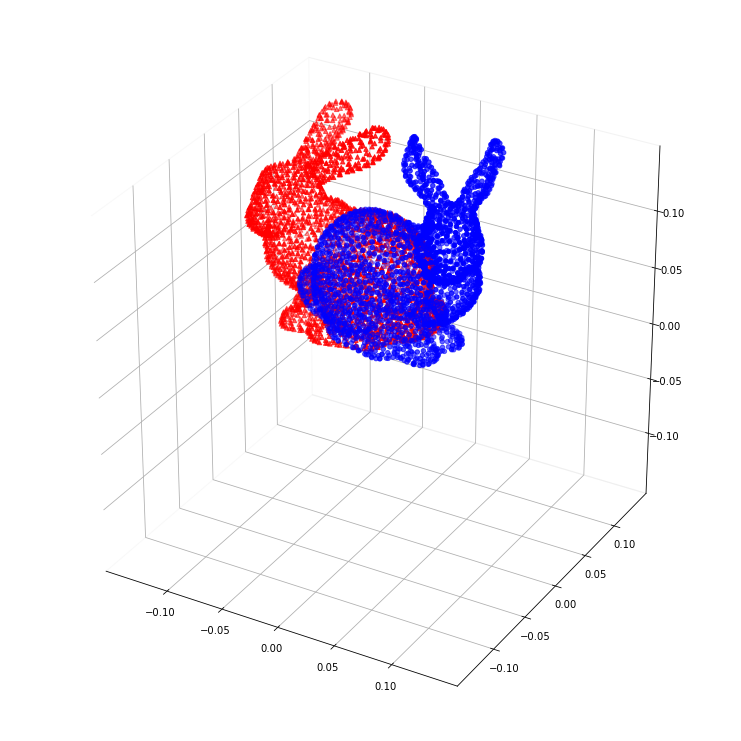
\includegraphics[width=\textwidth]{images/mirror_reflection_h}
      \caption{Дзеркальне відображення по горизонталі}
  \end{subfigure}
  \begin{subfigure}[b]{0.45\textwidth}
      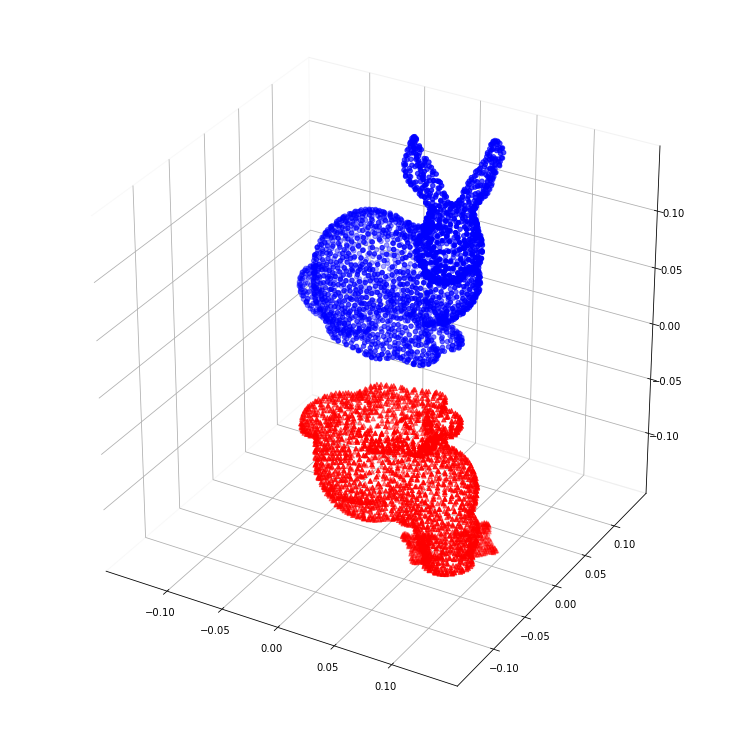
\includegraphics[width=\textwidth]{images/mirror_reflection_v}
      \caption{Дзеркальне відображення по вертикалі}
  \end{subfigure}
  \caption{Приклади дзеркальних відображень}
  \label{fig:mirror:reflection}
\end{figure}

Припустимо, що $ \det{ \left( V \cdot U^T \right) } = -1$.
Це еквівалентно тому, що
\begin{equation*}
  \det{M} =
  -1.
\end{equation*}
Шукаємо таку матрицю $M$, яка максимізує вираз
\begin{equation*}
  tr \left( \Sigma \cdot M \right) =
  \sigma_1 \cdot m_{11} + \sigma_2 \cdot m_{22} + \sigma_3 \cdot m_{33}.
\end{equation*}
Розглядаємо вектор $ \left( m_{11}, m_{22}, m_{33} \right) \in \mathbb{R}^3$.
Це множина всіх діагоналей ортогональної матриці порядка $3$.
Альфред Хорн довів \cite{horn:diagonal:rotation},
що вектор $ \left( d_1, \dotsc, d_n \right) $~---~це діагональ матриці повороту
порядка  $n$ тоді й тільки тоді,
коли він лежить у випуклій оболонці точок $ \left( \pm 1, \dotsc, \pm 1 \right) $,
де парне число значень (в тому числі жодне) дорівнює $-1$.
Для нашого випадку ця теорема приймає такий вигляд:
$M$~---~матриця повороту тоді й тільки тоді,
коли її діагональ $ \left( m_{11}, m_{22}, m_{33} \right) $ лежить у випуклій оболонці точок
$ \left( \pm 1, \pm 1, \pm 1 \right) $, де парна кількість координат
(в тому числі жодна) дорівнює $-1$.
Матриця $M$~---~матриця повороту та дзеркального відображення,
тому для неї оптимальна діагональ має вигляд $ \left( 1, 1, -1 \right) $,
коли непарна кількість значень дорівнює $-1$, відповідно,
\begin{equation*}
  tr \left( \Sigma \cdot M \right) = \sigma_1 + \sigma_2 - \sigma_3.
\end{equation*}
Це значення більше будь-якого іншого вектора з
$ \left( \pm 1, \pm 1, \pm 1 \right) $ за виключенням
$ \left( 1, 1, 1 \right) $, бо $ \sigma_3$~---~це найменше сингулярне значення.

Таким чином, якщо $ \det{ \left( V \cdot U^T \right) } = -1$, то
\begin{equation*}
  M =
  V^T \cdot R \cdot U =
  \begin{bmatrix}
    1 & 0 & 0 \\
    0 & 1 & 0 \\
    0 & 0 & -1
  \end{bmatrix} \Rightarrow
  R =
  V \cdot
  \begin{bmatrix}
    1 & 0 & 0 \\
    0 & 1 & 0 \\
    0 & 0 & -1
  \end{bmatrix} \cdot U^T.
\end{equation*}

Таким чином, шукана матриця повороту $R$ має вигляд  \cite{svd}
\begin{equation}\label{eq:estimated:R}
  R =
  V \cdot
  \begin{bmatrix}
    1 & 0 & 0 \\
    0 & 1 & 0 \\
    0 & 0 & \det{ \left( V \cdot U^T \right) }
  \end{bmatrix} \cdot U^T,
\end{equation}
а оптимальний вектор зсуву обчислюється за формулою \eqref{eq:translation}.

Отже, ітеративний алгоритм найближчих точок полягає в почерговому виконанні
двох кроків:
\begin{enumerate}
  \item пошук найкращої розмітки $k$ при фіксованих $R$ і $\boldsymbol{b}$;
  \item пошук матриці повороту $R$ і вектора зсуву $ \boldsymbol{b}$
  при фіксованій розмітці $k$,
  \item перші два кроки повторюються один за одним,
  поки не буде досягнений мінімум в \eqref{eq:least:squares}.
\end{enumerate}

\section{Збіжність алгоритму}

\textbf{Теорема.}
Ітеративний алгоритм найближчих точок завжди збігається.

Припустимо, що алгоритм нікуди не збігається.
Тоді існує така скінченна множина $S$, матриця повороту $R$,
вектор зсуву $ \boldsymbol{b}$ та шум $ \boldsymbol{ \xi_s}$,
що алгоритм буде виконувати нескінченно багато ітерацій і ніколи не зупиниться.

Нехай алгоритм перебрав усі можливі розмітки,
тобто виконав $ \left| T \right|^{ \left| S \right| }$ ітерацій, і не зупинився.
В цьому випадку на наступній ітерації буде вибрана розмітка,
яка вже вибиралась на одній з попередніх ітерацій.
Тоді вираз \eqref{eq:least:squares} або збільшиться
(що неможливо за побудовою алгоритму),
або не зміниться, і алгоритм закінчить свою роботу.
Це означає, що алгоритм завжди збігається.

\section{Розподіл оцінок}

\subsection{Теорема про незалежність елементів матриці $X$}

\textbf{Теорема}.
Асимптотично матриця $X = \tilde{S} \cdot \tilde{K}^T = U \cdot \Sigma \cdot V^T$
має нормальний розподіл, причому елементи матриці незалежні.

Те, що елементи матриці $X$ мають нормальний розподіл,
випливає з \eqref{eq:normal}.
Доведемо незалежність.
Для цього знайдемо кореляцію двох довільних елементів матриці $X$
\begin{equation}\label{eq:cor}
  cor \left( x_{ij}, x_{kr} \right) =
  \frac{cov \left( x_{ij}, x_{kr} \right) }{\sqrt{Dx_{ij} \cdot Dx_{kr}}},
\end{equation}
де $i, k$~---~індекси рядків матриці $X$,
а $j, r$~---~індекси стовпців матриці $X$.
Знайдемо окремо вираз у чисельнику
\begin{equation*}
  cov \left( x_{ij}, x_{kr} \right) =
  cov \left[
    \sum \limits_{t=1}^n \tilde{s}_{ti} \cdot \left(
      \xi_{s_t i}^T - \frac{1}{n} \sum \limits_{p=1}^n \xi_{s_p j}^T
    \right),
    \sum \limits_{q=1}^n \tilde{s}_{qk} \cdot \left(
      \xi_{s_q r}^T - \frac{1}{n} \sum \limits_{g=1}^n \xi_{s_g r}^T
    \right)
  \right].
\end{equation*}
Винесемо суми та константи
\begin{equation*}
  cov \left( x_{ij}, x_{kr} \right) =
  \sum \limits_{t=1}^n
    \sum \limits_{q=1}^n
      \tilde{s}_{ti} \cdot \tilde{s}_{qk} \cdot cov \left(
        \xi_{s_t j}^T - \frac{1}{n} \sum \limits_{p=1}^n \xi_{s_p j}^T,
        \xi_{s_q r}^T - \frac{1}{n} \sum \limits_{g=1}^n \xi_{s_g r}^T
      \right).
\end{equation*}
Розкриємо дужки
\begin{equation*}
  \begin{gathered}
    cov \left( x_{ij}, x_{kr} \right) =
    \sum \limits_{t=1}^n
      \sum \limits_{q=1}^n
        \tilde{s}_{ti} \cdot \tilde{s}_{qk} \cdot
        cov \left( \xi_{s_t j}^T, \xi_{s_q r}^T \right) + \\
    + \sum \limits_{t=1}^n
      \sum \limits_{q=1}^n
        \tilde{s}_{ti} \cdot \tilde{s}_{qk} \cdot cov \left(
          \xi_{s_t j}^T, -\frac{1}{n} \sum \limits_{g=1}^n \xi_{s_g r}^T
        \right) + \\
    + \sum \limits_{t=1}^n
      \sum \limits_{q=1}^n
        \tilde{s}_{ti} \cdot \tilde{s}_{qk} \cdot cov \left(
          -\frac{1}{n} \sum \limits_{p=1}^n \xi_{s_p j}^T, \xi_{s_1 r}^T
        \right) + \\
    + \sum \limits_{t=1}^n
      \sum \limits_{q=1}^n
        \tilde{s}_{ti} \cdot \tilde{s}_{qk} \cdot cov \left(
          -\frac{1}{n} \sum \limits_{p=1}^n \xi_{s_p j}^T,
          -\frac{1}{n} \sum \limits_{g=1}^n \xi_{s_g r}^T
        \right) \equiv
    A + B + C + D,
  \end{gathered}
\end{equation*}
де через $A, B, C, D$ позначені доданки.
Обчислимо кожний з них окремо.
Почнемо з першого доданку
\begin{equation*}
  A =
  \begin{cases}
    \sum \limits_{t=1}^n \tilde{s}_{ti} \cdot \tilde{s}_{tk} \cdot \sigma^2 =
    \sigma^2 \sum \limits_{t=1}^n \tilde{s}_{ti} \cdot \tilde{s}_{tk},
    \qquad j = r, \\
    0,\ \qquad j \neq r.
  \end{cases}
\end{equation*}
Другий доданок
\begin{equation*}
  B =
  -\frac{1}{n} \sum \limits_{t=1}^n
    \sum \limits_{q=1}^n
      \tilde{s}_{ti} \cdot \tilde{s}_{qk} \sum \limits_{g=1}^n
        cov \left( \xi_{s_t j}^T, \xi_{s_g r}^T \right) =
  \begin{cases}
    -\frac{\sigma^2}{n} \sum \limits_{t=1}^n
      \sum \limits_{q=1}^n \tilde{s}_{ti} \cdot \tilde{s}_{qk}, \qquad j = r, \\
    0, \qquad j \neq r.
  \end{cases}
\end{equation*}
Третій доданок
\begin{equation*}
  C =
  -\frac{1}{n} \sum \limits_{t=1}^n
    \sum \limits_{q=1}^n
      \tilde{s}_{ti} \cdot \tilde{s}_{qk} \sum \limits_{p=1}^n
        cov \left( \xi_{s_p j}^T, \xi_{s_q r}^T \right) =
  \begin{cases}
    -\frac{\sigma^2}{n} \sum \limits_{t=1}^n \sum \limits_{q=1}^n
      \tilde{s_{ti}} \cdot \tilde{s}_{qk}, \qquad j = r, \\
    0, \qquad j \neq r.
  \end{cases}
\end{equation*}
Четвертий доданок
\begin{equation*}
  \begin{gathered}
    D =
    \frac{1}{n^2} \sum \limits_{t=1}^n
      \sum \limits_{q=1}^n
        \tilde{s}_{ti} \cdot \tilde{s}_{qk} \sum \limits_{p=1}^n
          \sum \limits_{g=1}^n cov \left( \xi_{s_p j}^T, \xi_{s_g r}^T \right) = \\
    = \begin{cases}
      \frac{\sigma^2}{n^2} \sum \limits_{t=1}^n
        \sum \limits_{q=1}^n \tilde{s}_{ti} \cdot \tilde{s}_{qk} \cdot n =
      \frac{\sigma^2}{n} \sum \limits_{t=1}^n
        \sum \limits_{q=1}^n \tilde{s}_{ti} \cdot \tilde{s}_{qk}, \qquad j = r, \\
      0, \qquad j \neq r.
    \end{cases}
  \end{gathered}
\end{equation*}
Бачимо, що другий і третій доданки рівні,
а четверний співпадає з ними з протилежним знаком.
Отже, отримуємо
\begin{equation*}
  cov \left( x_{ij}, x_{kr} \right) =
  A + B =
  \begin{cases}
    \sigma^2 \sum \limits_{t=1}^n \tilde{s}_{ti} \cdot \tilde{s}_{tk} -
    \frac{\sigma^2}{n} \sum \limits_{t=1}^n
      \sum \limits_{q=1}^n \tilde{s}_{ti} \cdot \tilde{s}_{qk}, \qquad j = r, \\
    0, \qquad j \neq r.
  \end{cases}
\end{equation*}

Знайдемо дисперсію
\begin{equation*}
  \begin{gathered}
    Dx_{ij} =
    D \left[
      \sum \limits_{t=1}^n \tilde{s}_{ti} \cdot \left(
        \xi_{s_t j}^T - \frac{1}{n} \sum \limits_{p=1}^n \xi_{s_p j}^T
      \right) \right] = \\
    = \sum \limits_{t=1}^n \tilde{s}_{ti}^2 \cdot \left[ D \xi_{s_t j}^T + D \left(
      -\frac{1}{n} \sum \limits_{p=1}^n
        \xi_{s_p j})^T \right) + 2cov \left( \xi_{s_t j}^T,
      -\frac{1}{n} \sum \limits_{p=1}^n \xi_{s_p j}^T
    \right) \right] = \\
    = \sum \limits_{t=1}^n \tilde{s}_{ti}^2 \cdot \left(
      \sigma^2 + \frac{\sigma^2}{n} - \frac{2 \sigma^2}{n}
    \right) =
    \sigma^2 \sum \limits_{t=1}^n \tilde{s}_{ti}^2 \cdot
    \left( 1 - \frac{1}{n} \right).
  \end{gathered}
\end{equation*}
Аналогічно,
\begin{equation*}
  Dx_{kr} =
  \sigma^2 \sum \limits_{t=1}^n
    \tilde{s}_{tk} \cdot \left( 1 - \frac{1}{n} \right).
\end{equation*}

Підставимо отримані вирази в формулу для кореляції \eqref{eq:cor}
\begin{equation}\label{eq:corto}
  \begin{gathered}
    cor \left( x_{ij}, x_{kr} \right) =
    \frac{\sigma^2 \left( \sum \limits_{t=1}^n \tilde{s}_{ti} \cdot \tilde{s}_{tk} - \frac{1}{n} \sum \limits_{t=1}^n \sum \limits_{q=1}^n \tilde{s}_{ti} \cdot \tilde{s}_{qk} \right) }{\left[ \sigma^2 \sum \limits_{t=1}^n \tilde{s}_{ti}^2 \cdot \left( 1 - \frac{1}{n}\right) \cdot \sigma^2 \sum \limits_{q=1}^n \tilde{s}_{qk}^2 \cdot \left( 1 - \frac{1}{n} \right)\right]^{\frac{1}{2}}} \leq \\
    \leq \frac{\left| \sum \limits_{t=1}^n \tilde{s}_{ti} \cdot \tilde{s}_{tk} - \frac{1}{n} \sum \limits_{t=1}^n \sum \limits_{q=1}^n \tilde{s}_{ti} \cdot \tilde{s}_{qk} \right|}{ \frac{n-1}{n} \cdot \left( \sum \limits_{t=1}^n \tilde{s}_{ti}^2 \sum \limits_{q=1}^n \tilde{s}_{qk}^2\right)^{\frac{1}{2}}} \leq
    \frac{\left| \sum \limits_{t=1}^n \tilde{s}_{ti} \cdot \tilde{s}_{tk}\right|+ \frac{1}{n} \cdot \left| \sum \limits_{t=1}^n \sum \limits_{q=1}^n \tilde{s}_{ti} \cdot \tilde{s}_{qk}\right|}{\frac{n-1}{n} \cdot \left(\sum \limits_{t=1}^n \tilde{s}_{ti}^2 \sum \limits_{q=1}^n \tilde{s}_{qk}^2\right)^{\frac{1}{2}}}.
  \end{gathered}
\end{equation}
Поділимо почленно чисельник на знаменник та розглянемо окремо перший доданок.
Використовуємо нерівність Коші-Буняковського \cite{DorogovtsevMA}
\begin{equation*}
  \frac{\left| \sum \limits_{t=1}^n \tilde{s}_{ti} \cdot \tilde{s}_{tk}\right|}{\frac{n-1}{n} \cdot \sqrt{\sum \limits_{t=1}^n \tilde{s}_{ti}^2 \sum \limits_{q=1}^n \tilde{s}_{qk}^2}} \leq
  \frac{\sqrt{\sum \limits_{t=1}^n \tilde{s}_{ti}^2 + \sum \limits_{t=1}^n \tilde{s}_{tk}^2}}{\frac{n-1}{n} \cdot \sqrt{\sum \limits_{t=1}^n \tilde{s}_{ti}^2 \sum \limits_{q=1}^n \tilde{s}_{qk}^2}}\leq
  \frac{\sqrt{\sum \limits_{t=1}^n \left( \tilde{s}_{ti} + \tilde{s}_{tk} \right)^2}}{\frac{n-1}{n} \cdot \sqrt{\sum \limits_{t=1}^n \tilde{s}_{ti}^2 \sum \limits_{q=1}^n \tilde{s}_{qk}^2}}.
\end{equation*}
Згідно з нерівністю Мінковського \cite{DorogovtsevMA} цей вираз не перевищує
\begin{equation*}
  \frac{\sqrt{\sum \limits_{t=1}^n \tilde{s}_{ti}^2} + \sqrt{\sum \limits_{t=1}^n \tilde{s}_{tk}^2}}{\frac{n-1}{n} \cdot \sqrt{\sum \limits_{t=1}^n \tilde{s}_{ti}^2 \sum \limits_{q=1}^n \tilde{s}_{qk}^2}} =
  \frac{1}{\left( 1 - \frac{1}{n}\right) \cdot \sqrt{\sum \limits_{t=1}^n \tilde{s}_{tk}^2}} + \frac{1}{\left( 1 - \frac{1}{n} \right) \cdot \sqrt{\sum \limits_{t=1}^n \tilde{s}_{ti}^2}}.
\end{equation*}

У вихідній задачі треба знайти функцію перетворення множини точок
$\tilde{\boldsymbol{s}}$.
Її прообраз~---~точкова множина $\tilde{S}$.
Тому чим більше точок міститься в прообразі функції перетворення,
тим точніше можна відновити цю функцію.
Тобто з ростом $n$ сума квадратів координат точок множини $\tilde{S}$
буде тільки збільшуватись.
Отже, вираз \eqref{eq:corto} прямує до нуля при $n \to \infty $.

Розглянемо другий доданок у виразі \eqref{eq:corto}
\begin{equation*}
  \frac{\left| \sum \limits_{t=1}^n \sum \limits_{q=1}^n \tilde{s}_{ti} \cdot \tilde{s}_{qk} \right|}{\left(n-1\right) \cdot \sqrt{\sum \limits_{t=1}^n \tilde{s}_{ti}^2 \sum \limits_{q=1}^n \tilde{s}_{qk}^2}} \leq
  \frac{1}{n-1}\cdot \frac{\frac{1}{n}\sum \limits_{t=1}^n \left|\tilde{s}_{ti} \right| \cdot \frac{1}{n} \sum \limits_{q=1}^n \left| \tilde{s}_{qk} \right| \cdot n^2}{\sqrt{\frac{1}{n}\sum \limits_{t=1}^n \tilde{s}_{ti}^2 \cdot \frac{1}{n}\sum \limits_{q=1}^n \tilde{s}_{qk}^2} \cdot n^4}.
\end{equation*}
Використаємо нерівність між середнім квадратичним та середнім арифметичним.
Бачимо, що наступний вираз не менше попереднього
\begin{equation*}
  \frac{1}{n - 1} \cdot \frac{\frac{1}{n} \sum \limits_{t=1}^n \left| \tilde{s}_{ti} \right| \cdot \frac{1}{n} \sum \limits_{q=1}^n \left| \tilde{s}_{qk} \right|}{\frac{1}{n} \sum \limits_{t=1}^n \left| \tilde{s}_{ti} \right| \cdot \frac{1}{n} \sum \limits_{q=1}^n \left| \tilde{s}_{qk} \right| \cdot n^2} =
  \frac{1}{n^2 \cdot \left( n-1 \right)} \to
  0, \, n \to \infty.
\end{equation*}
Доведення теореми завершено.
Отже, в асимптотиці елементи матриці $X$ незалежні.

\subsection{Розподіл матриць $U$ та $V$ в сингулярному розкладі матриці $X$}

Запишемо розподіл ймовірностей елементів матриці $X$
\begin{equation*}
  \begin{gathered}
    \prod \limits_{i=1}^9 \frac{1}{\sqrt{2 \pi}} \cdot e^{x_i^2} dx_i =
    \frac{1}{\left( \sqrt{2 \pi} \right)^9} \cdot
    e^{-\frac{1}{2} \sum \limits_{i=1}^9 x_i^2}
    dx_1 \cdot \dotsc \cdot dx_9 = \\
    = \frac{1}{\left( \sqrt{2 \pi} \right)^9} \cdot
    e^{-\frac{1}{2} \cdot tr \left( X \cdot X^T \right)} dX.
  \end{gathered}
\end{equation*}
Зробимо заміну $X = U \cdot \Sigma \cdot V^T$
та скористаємось властивістю сліду \eqref{eq:trace}
\begin{equation*}
  \begin{gathered}
  \frac{1}{ \left( \sqrt{2 \pi}\right)^9} \cdot
  \exp{\left\{ -\frac{1}{2} \cdot tr \left(
    U \cdot \Sigma \cdot V^T \cdot V \cdot \Sigma^T \cdot U^T
  \right)\right\}} dX = \\
  = \frac{1}{\left( \sqrt{2 \pi} \right)^9} \cdot
  e^{-\frac{1}{2} \cdot tr \left( \Sigma^T \cdot \Sigma \right)} dX.
  \end{gathered}
\end{equation*}
Диференціали $dX$ та $dU d \Sigma dV$ пов'язані співвідношенням \cite{jacobians}
\begin{equation*}
  dX =
  \prod \limits_{1 \leq i < j \leq 3} \left( \sigma_i^2 - \sigma_j^2 \right)
  d \Sigma dU dV.
\end{equation*}
Таким чином, розподіл ймовірностей елементів матриці $X$ має вигляд
\begin{equation*}
  \frac{1}{\left( \sqrt{2 \pi}\right)^9} \cdot
  e^{-\frac{1}{2} \cdot tr \left( \Sigma^T \cdot \Sigma \right) }
  \prod \limits_{1 \leq i < j \leq 3} \left( \sigma_i - \sigma_j \right)
  d \Sigma dU dV.
\end{equation*}
Останній вираз~---~це добуток трьох розподілів ймовірностей \cite{jacobians}:
\begin{equation*}
  e^{-\frac{1}{2} \cdot tr \left( \Sigma^T \cdot \Sigma \right) }
  \prod \limits_{1 \leq i < j \leq 3} \left( \sigma_i - \sigma_j \right)
  d \Sigma
\end{equation*}
для матриці $\Sigma$, $dU$ для матриці $U$ та $dV$ для матриці $V$
з точністю до констант.
Отже, елементи матриць $U$ та $V$ незалежні та мають рівномірний розподіл.

\subsection{Розподіл елементів матриці повороту на кожній ітерації}

Шукаємо розподіл елементів матриці $R = V \cdot U^T$, де
\begin{equation*}
  r_{ij} =
  \sum \limits_{s = 1}^3 v_{is} \cdot u_{sj}^T =
  \sum \limits_{s = 1}^3 r_s.
\end{equation*}
Щільність розподілу випадкових величин $v_{is}$ та $u_{sj}^T$,
які мають рівномірний розподіл на відрізку $\left[ -1, 1 \right] $
\begin{equation*}
  p_{v_{is}} \left( x \right) =
  p_{u_{sj}^T} \left( x \right) =
  \frac{1}{2} \cdot \mathbbm{1} \left\{ x \in \left[ -1, 1 \right] \right\}.
\end{equation*}
При цьому модулі випадкових величин $v_{is}$ та $u_{sj}^T$
мають стандартний рівномірний розподіл
\begin{equation*}
  p_{\left| v_{is} \right|} \left( x \right) =
  p_{\left| u_{sj}^T \right|} \left( x \right) =
  \mathbbm{1} \left\{ x \in \left[ 0, 1 \right] \right\}.
\end{equation*}
Знайдемо розподіл величини
$ \left| r_s \right| = \left| v_{is} \right| \cdot \left| u_{sj}^T \right|$.
Візьмемо логарифм від правої і лівої частин останньої рівності
\begin{equation*}
  \ln \left| r_s \right| = \ln \left| v_{is} \right| + \ln \left| u_{sj}^T \right|.
\end{equation*}
Так як випадкові величини $v_{is}$ і $u_{sj}^T$~---~незалежні, то $\ln \left| v_{is} \right|$ і
$\ln \left| u_{sj}^T \right|$~---~теж незалежні.
Виразимо функції розподілу логарифмів модулів випадкових величин
\begin{equation*}
  F_{ln \left| v_{is} \right|} \left( x \right) =
  P \left( \ln \left| v_{is} \right| \leq x \right) =
  P \left( \left| v_{is} \right| \leq e^x \right) =
  F_{\left| v_{is} \right|} \left( e^x \right).
\end{equation*}
Тоді щільність розподілу
\begin{equation*}
  p_{\ln \left| v_{is} \right|} \left( x \right) =
  \left[ F_{\ln \left| v_{is} \right|} \left( x \right) \right]' =
  e^x \cdot p_{\left| v_{is} \right|} \left( e^x \right) =
  e^x \cdot \mathbbm{1} \left\{ e^x \in \left[ 0, 1 \right] \right\} =
  e^x \cdot \mathbbm{1} \left\{ x \leq 0 \right\}.
\end{equation*}
Аналогічно,
\begin{equation*}
  p_{\ln \left| u_{sj}^T \right|} \left( x \right) =
  e^x \cdot \mathbbm{1} \left\{ x \leq 0 \right\}.
\end{equation*}
Отримуємо щільність розподілу суми незалежних випадкових величин
\begin{equation*}
  \begin{gathered}
    p_{\ln \left| r_s \right|} \left( x \right) =
    \int \limits_{-\infty }^{+\infty }
      p_{\ln \left| v_{is} \right|}\left( x - y \right) \cdot
      p_{\ln \left| u_{sj}^T\right|}
    dy = \\
    = \int \limits_{-\infty}^{+\infty}
      e^{x-y} \cdot \mathbbm{1} \left\{ x - y \leq 0 \right\} \cdot
      e^y \cdot \mathbbm{1} \left\{ y \leq 0 \right\}
    dy =
    e^x \int \limits_{\min \left( x, 0 \right)}^0 dy =
    -e^x \cdot \min \left( x, 0 \right).
  \end{gathered}
\end{equation*}
Перейдемо від розподілу логарифму випадкової величини $ \ln \left| r_s \right|$
до розподілу самої випадкової величини $\left| r_s \right|$
\begin{equation*}
  p_{\left| r_s \right|} \left( x \right) =
  \frac{1}{x} \cdot p_{\ln \left| r_s \right|} \left( \ln \, x \right) =
  -\frac{1}{x} \cdot e^{\ln \, x} \cdot \min \left( \ln\, x, 0 \right) =
  -\ln \, x, \, 0 \leq x \leq 1.
\end{equation*}
Замінюємо $x$ на $\left| x \right| $ в останньому виразі та ділимо його на $2$,
щоб отримати щільність розподілу випадкової величини $r_s$.
Маємо
\begin{equation*}
  p_{r_s} \left( x \right) =
  -\frac{1}{2} \cdot
  \ln \left| x \right| \cdot \mathbbm{1} \left\{ x \in \left[ -1, 1 \right] \right\}.
\end{equation*}

Знайдемо математичне сподівання цієї випадкової величини
\begin{equation*}
  Mr_s =
  \int \limits_{-\infty}^{+\infty} x \cdot p \left( x \right) dx =
  -\frac{1}{2} \int \limits_{-1}^1 x \cdot \ln \left| x \right| dx =
  -\frac{1}{2} \cdot
  \left. \ln \left| x \right| \cdot \frac{x^2}{2} \right|_{-1}^1 +
  \frac{1}{2} \int \limits_{-1}^1 \frac{x^2}{2} \cdot \frac{1}{x} dx =
  0.
\end{equation*}

Тоді математичне сподівання елементу знайденої матриці повороту $R$
\eqref{eq:estimated:R} дорівнює
$Mr_{ij} =
  M \left( r_1 + r_2 + r_3 \right) =
  0$.
Результат є очікуваним,
бо математичне сподівання ґаусового шуму \eqref{eq:problem} дорівнює нулю.
Тому при малих значеннях шуму поворот точок множини вихідної множини $S$ теж
буде малим.

\section{Простий приклад незадовільної роботи алгоритму}

На рисунку \ref{fig:triangles} зображено приклад двох множин,
для яких алгоритм не дає очікуваного результату.

\begin{figure}[h]
  \centering
  \includestandalone[mode=buildnew]{../tikz/triangles}
  \caption{Два трикутника, при співставленні яких ICP не дає очікуваного результату}
  \label{fig:triangles}
\end{figure}

Множини представляють собою два ідентичних прямокутник трикутника з катетами,
які дорівнюють одиниці, що відрізняються кутом повороту $\theta = \pi$ та зсувом
\begin{equation*}
  \boldsymbol{b} =
  \begin{bmatrix}
    \frac{ \sqrt{2}}{2} \\
    \frac{ \sqrt{2}}{2}
  \end{bmatrix} \approx
  \begin{bmatrix}
    0.7071 \\
    0.7071
  \end{bmatrix}.
\end{equation*}
Множину $S$ зображено пунктиром.
Це трикутник з вершинами
$ \left( 0, 0 \right), \left( 0, 1 \right) $ і $ \left( 1, 0 \right) $.
Множину $T$, яка складається з точок $\boldsymbol{t} = R \cdot \boldsymbol{s} + \boldsymbol{b}$,
зображено суцільною лінією, де $\boldsymbol{s}$~---~точки множини $S$,
а $R$~---~матриця повороту
\begin{equation*}
  R =
  \begin{bmatrix}
    \cos \theta & -\sin \theta \\
    \sin \theta & \cos \theta
  \end{bmatrix} =
  \begin{bmatrix}
    -1 & 0 \\
    0 & -1
  \end{bmatrix}.
\end{equation*}
Таким чином, множини $S$ і $T$ мають вигляд
\begin{equation*}
  S =
  \begin{bmatrix}
    0 & 0 & 1 \\
    0 & 1 & 0
  \end{bmatrix}, \,
  T =
  \begin{bmatrix}
    \frac{ \sqrt{2}}{2} & \frac{ \sqrt{2}}{2} & \frac{ \sqrt{2}}{2} - 1 \\
    \frac{ \sqrt{2}}{2} & \frac{ \sqrt{2}}{2} - 1 & \frac{ \sqrt{2}}{2}
  \end{bmatrix}.
\end{equation*}

До цих множин був застосований ітеративний алгоритм найближчих точок.
Алгоритм зупинився, виконавши дві ітерації, бо розмітка, знайдена на другій ітерації,
співпала з розміткою, знайденою на першій ітерації.
Отримані взаємні розміщення множин зображені на рисунку
\ref{fig:triangles_result}.

\begin{figure}[h]
  \centering
  \includestandalone[mode=buildnew]{../tikz/triangles_result}
  \caption{Результат ICP для трикутників}
  \label{fig:triangles_result}
\end{figure}

Оцінка матриці повороту та вектора зсуву
\begin{equation*}
  \hat{R} =
  \begin{bmatrix}
    0.9487  & 0.3162 \\
    -0.3162 & 0.9487
  \end{bmatrix}, \,
  \hat{\boldsymbol{b}} =
  \begin{bmatrix}
    0.0969 \\
    0.1939
  \end{bmatrix}.
\end{equation*}
Згідно алгоритму, кут повороту між множинами становить приблизно $18$ градусів.
Отримані значення параметрів сильно відрізняються від істинних,
що видно і на рисунку \ref{fig:triangles_result}.
Отже, алгоритм не зміг правильно оцінити кут повороту та зсув множини $T$
відносно множини $S$.

Правильним результатом були б такі поворот і зсув,
коли всі відповідні точки двох трикутників мали б однакові положення,
тобто коли трикутники повністю наклалися б один на одний.
Через те, що найближчі точки не є відповідними,
глобальний мінімум не досягається.

\section{Стенфордський кролик}

Для цього прикладу була використана тривимірна модель \cite{bunny},
що складається з $2503$ точок, створена Грегом Тюрком та Марком Левоєм в
Стенфордському університеті в 1994 році для тестування алгоритмів комп'ютерної
графіки, включаючи зменшення кількості полігонів,
стиснення даних та згладжування поверхонь.
Точки вихідної множини повернули відносно осі $z$ на $40$ градусів,
що становить $\theta = 0.6981$ радіани, та зсунули на $0.1$ в бік,
протилежний спостерігачеві.
При цьому розміри моделі по цій осі становлять приблизно $0.08$.
Матриця повороту та вектор зсуву мають вигляд
\begin{equation*}
  R = \begin{bmatrix}
    0.766  & -0.6428 & 0 \\
    0.6428 & 0.766   & 0 \\
    0      & 0       & 1
  \end{bmatrix}, \,
  \boldsymbol{b} =
  \begin{bmatrix}
    0 \\
    0 \\
    0.1
  \end{bmatrix}.
\end{equation*}
До точок вихідної множини також доданий ґаусів шум з нульовим математичним
сподіванням та дисперсією $0.001$.
Вихідна та отримана множини, тобто вхідні дані,
що подаються алгоритму на обробку, зображені на рисунку \ref{fig:bunny:input}.
Синім кольором зображена вихідна множина, а червоним~---~множина,
отримана після перетворення вихідної.
Назвемо її цільовою.

\begin{figure}[h]
  \centering
    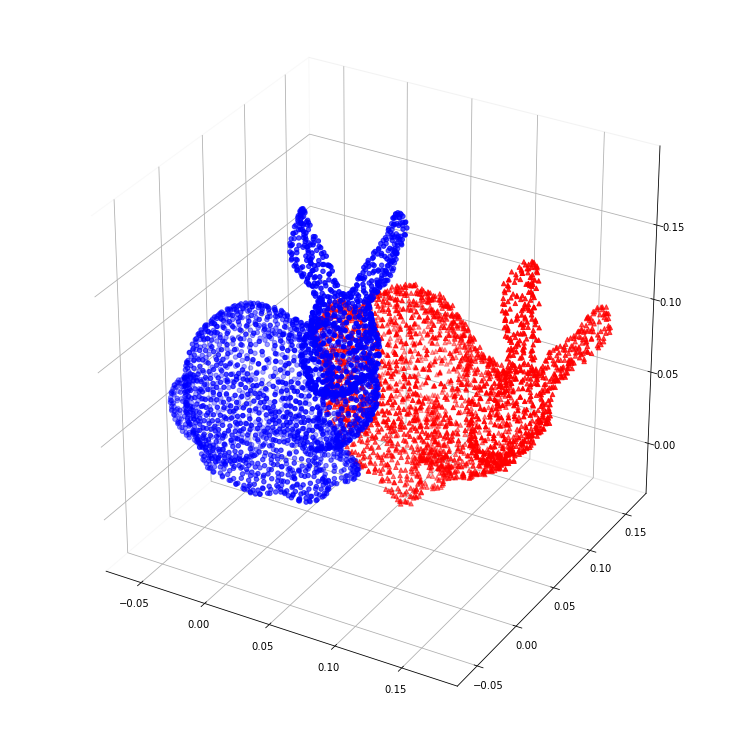
\includegraphics[width=0.9\textwidth]{images/bunny_input}
  \caption{Вхідні дані}
  \label{fig:bunny:input}
\end{figure}

Ці множини були співставлені за допомогою ітеративного алгоритму найближчих
точок.
На рисунку \ref{fig:bunny:iterations}
зображені ітерації роботи алгоритму на моделі кролика зі Стенфордського
університету.
Обрані ітерації кратні ступеню двійки, тому що так краще за все помітні зміни.

\begin{figure}[h]
  \centering
  \begin{subfigure}[b]{0.3\textwidth}
      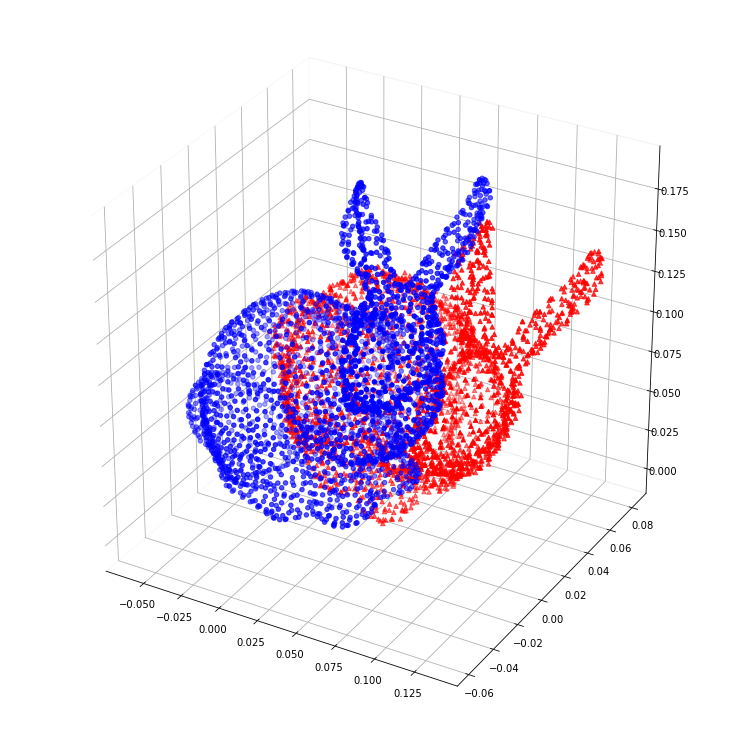
\includegraphics[width=\textwidth]{images/bunny_1}
      \caption{Ітерація 1}
  \end{subfigure}
  \begin{subfigure}[b]{0.3\textwidth}
      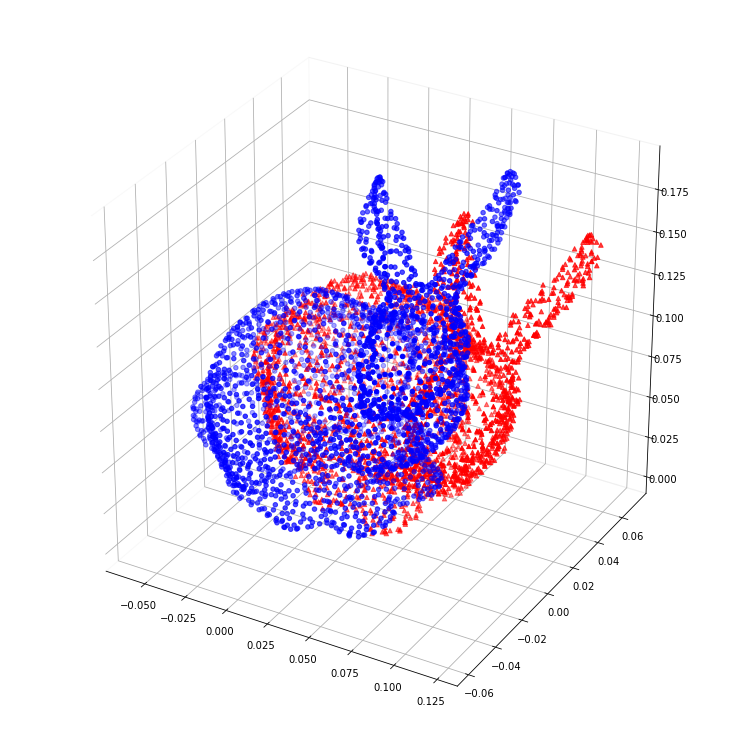
\includegraphics[width=\textwidth]{images/bunny_2}
      \caption{Ітерація 2}
  \end{subfigure}
  \begin{subfigure}[b]{0.3\textwidth}
      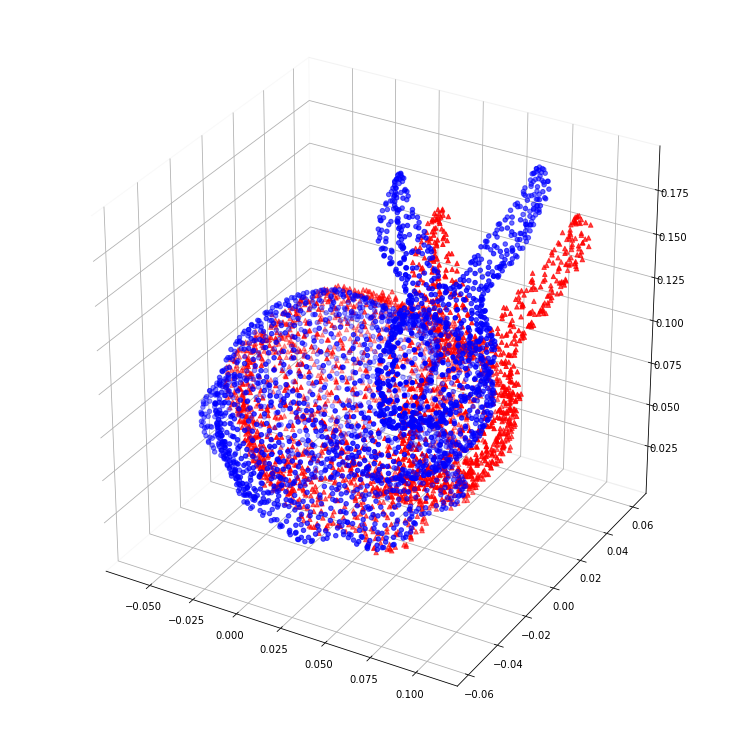
\includegraphics[width=\textwidth]{images/bunny_4}
      \caption{Ітерація 4}
  \end{subfigure}

  \begin{subfigure}[b]{0.4\textwidth}
      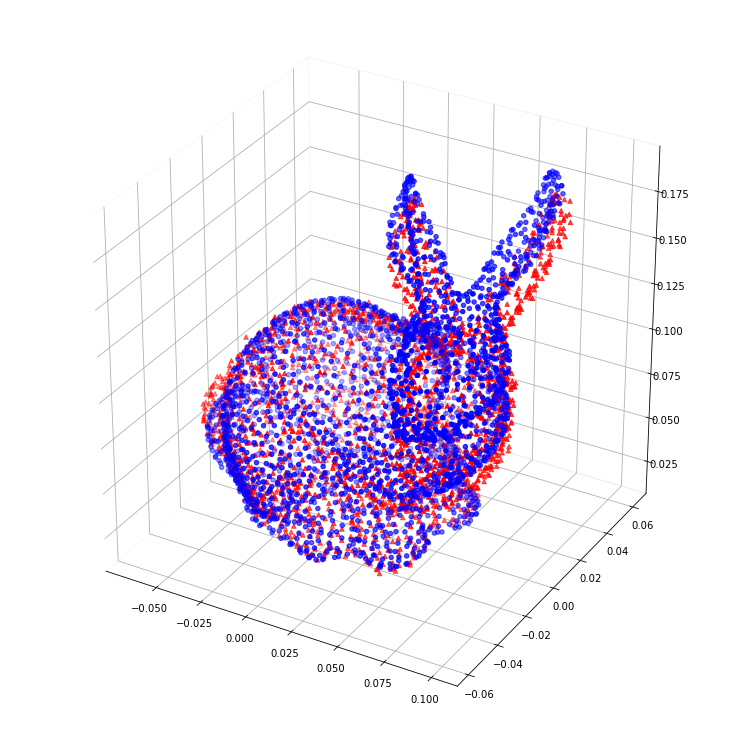
\includegraphics[width=\textwidth]{images/bunny_8}
      \caption{Ітерація 8}
  \end{subfigure}
  \begin{subfigure}[b]{0.4\textwidth}
      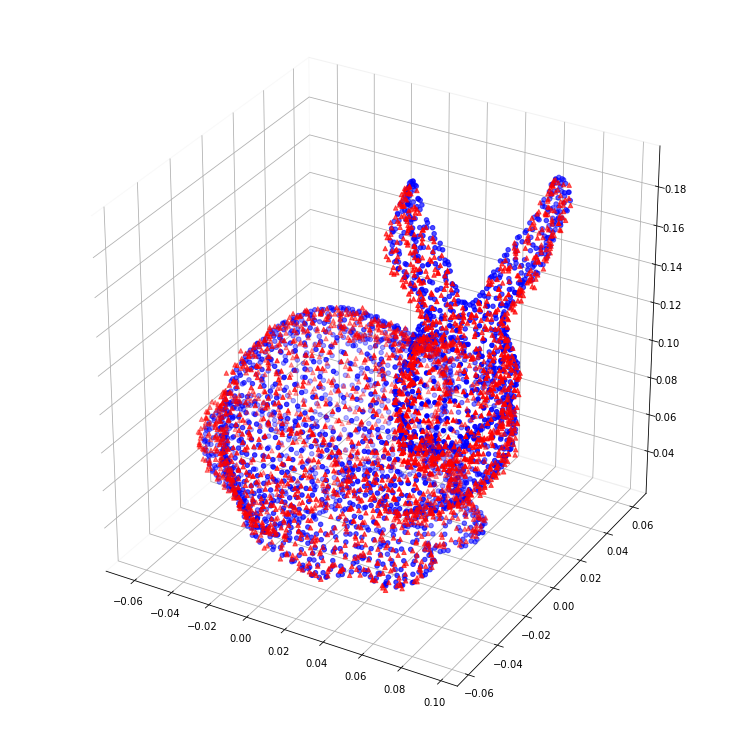
\includegraphics[width=\textwidth]{images/bunny_16}
      \caption{Ітерація 16}
  \end{subfigure}
  \caption{Результати проміжних ітерацій}
  \label{fig:bunny:iterations}
\end{figure}

Видно, що за декілька перших ітерацій алгоритм знайшов правильное розташування
вихідної множини відносно цільової,
а впродовж наступних ітерацій зміни в положенні вихідної множин, а отже,
і зміни в оцінках параметрів, були незначними.
Остаточний результат співставлення зображений на рисунку \ref{fig:bunny:result}.

\begin{figure}[h]
  \centering
    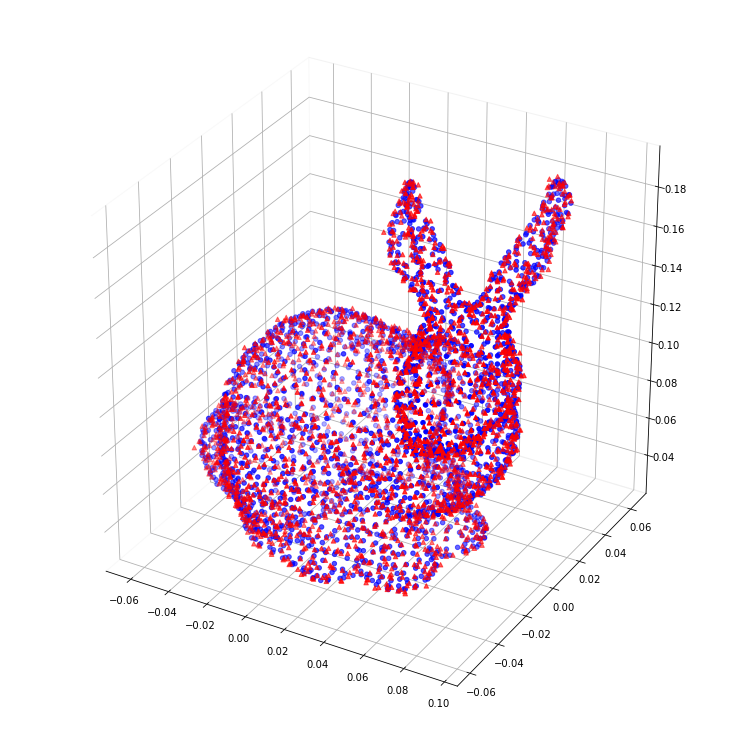
\includegraphics[width=0.9\textwidth]{images/bunny_result}
  \caption{Результат роботи алгоритму}
  \label{fig:bunny:result}
\end{figure}

Оцінка матриці повороту та вектора зсуву має вигляд
\begin{equation*}
  \hat{R} =
  \begin{bmatrix}
    0.7659  & -0.643  & 0 \\
    0.643   & 0.7659  & 0.0008 \\
    -0.0006 & -0.0006 & 1
  \end{bmatrix}, \,
  \hat{\boldsymbol{b}} =
  \begin{bmatrix}
    -0.0001 \\
    0 \\
    0.1
  \end{bmatrix}.
\end{equation*}
Знайдемо оцінку кута повороту
$\hat{\theta} = \arcsin \left( 0.643 \right) = 0.6984$ радіани,
що становить $40.0126$ градусів.
Порахуємо абсолютну похибку оцінки кута повороту в радіанах
\begin{equation*}
  \hat{\theta} - \theta =
  0.6984 - 0.6981 =
  0.0003.
\end{equation*}
Порахуємо відносну похибку оцінки кута повороту в радіанах
\begin{equation*}
  \Delta_{\theta} =
  \frac{\Delta}{\theta} \cdot 100 \%=
  \frac{0.0003}{0.6981} \cdot 100 \% =
  0.043 \%.
\end{equation*}
Відносна похибка дуже мала, отже, алгоритм відпрацював дійсно добре.
Такого результату вдалося досягти за $524$ мілісекунди на компьютері з
процесором Intel Core i5-3317U, виконавши $28$ ітерацій алгоритму.
Програмне забезпечення будо написано на Pyhton $2.7$ спеціально для цієї роботи.

\section*{Висновки до розділу 3}
\addcontentsline{toc}{section}{Висновки до розділу 3}

Проведено теоретичний опис ітеративного алгоритму найближчих точок для
розв'язання задачі, поставленої в першому розділі.
Алгоритм базується на обчисленні сингулярного розкладу певної матриці,
тому що цей підхід дає змогу отримати матрицю повороту.
Виявилося, що в даному випадку сингулярний розклад єдиний з точністю по
перестановки знаків.
Отже, невідомі параметри оцінюються однозначно.
Знайдено розподіл оцінки матриці повороту та доведено,
що алгоритм завжди зупиняється за скінченну кількість ітерацій.

Для деяких вхідних даних алгоритм дає дуже добрі результати, однак,
був знайдений простий приклад, для якого алгоритм не працює задовільно.
Таким чином, необхідні подальші дослідження,
щоб виявити ще слабкі та сильні сторони алгоритму.
